%\documentclass[aps, twocolumn, superscriptaddress, showpacs, linenumbers, nofootinbib]{revtex4-1}
\documentclass[aps, twocolumn, superscriptaddress, showpacs, nofootinbib, longbibliography]{revtex4-1}

% \documentclass[aps,prl,reprint,showpacs]{revtex4-1}

%\usepackage{lipsum}
\usepackage[utf8]{inputenc}
\usepackage[T1]{fontenc}
\usepackage{ae,aecompl} 
\usepackage{graphicx}
\usepackage{amsmath}
\usepackage{color}
\usepackage{amssymb}
\usepackage{latexsym}
\usepackage{wasysym}
\usepackage{psfrag}
%\usepackage{comment}
\usepackage{ifthen}
\usepackage[citecolor=blue,colorlinks=true]{hyperref}
\usepackage{longtable}
\usepackage{float}
\usepackage[utf8]{inputenc}
\usepackage{lineno}
%\usepackage{ulem}
%\usepackage{subfigure}
\newcommand{\note}[1]{{\color{red}#1}}
\newcommand{\second}{\ensuremath{\mathrm{\,s}}}


% \usepackage{svn-multi}
%\restylefloat{table}

\begin{document}
\linenumbers

\title{Identification of protoneutron star g-modes in gravitational-wave data}

\begin{abstract}

\end{abstract}

\maketitle

\section{Introduction}


The life of massive stars ($8 {\rm M}_\odot-100{\rm M}_\odot$) ends with the collapse of their iron core under their own gravity, leading the formation of a neutron star or a black hole (BH), followed (typically but not necessarily in the BH case) by the explosion of the star as a supernova. Core-collapse supernova (CCSN) explosions are one of the expected sources of gravitational-waves (GW) that have not yet been detected by current ground-based observatories. This is because even the most common type of CCSN, the neutrino-driven explosion, have a rate about three per century \cite{Gossan:2016} within our galaxy. The other main type of explosion, the magneto-rotational mechanism, can produce a more powerful signal and can be detected at distances up to $\sim 5$ Mpc \cite{Gossan:2016} \textcolor{red} Add better reference. However, the rate of events of this kind is much lower than the one for the neutrino driven mechanism $\sim 10^{-4} \rm{yr}^{-1}$, which represents less than $1 \%$ of all CCSNe.
Despite all this, collapsing stars produces a complex GW signal which could provide significant clues about the physical processes that occur in the moments after the collapse. 

In the past years impressive progresses have been made in the development of numerical codes, which allow to obtain more accurate CCSN simulations. The waveforms produced by the magneto-rotational mechanism in particular is well understood. The core-bounce signal can be directly related with the rotational properties of the core \cite{Dimmelmeier:2007, abdikamalov:14, Richers:2017}. However, the low rate of this kind of events and its expected low amplitude in the slow-rotation case, will probably impede its detection.

In the case of the neutrino-driven explosion mechanism, the GW emission is mainly produced during the hydrodynamical bounce and the unstable evolution of the fluid inside the region formed by the recently formed proto-neutron star (PNS) and the accretion shock. The dynamics excite the different modes of oscillation of the PNS \cite{kokkotas, Friedman:2013}. Unluckily, in this case it is not posible to relate the GW emission with the properties (mass, rotation rate, metallicity or magnetic fields) of the progenitor stars.  A large number of physical processes are involved and their role is not completely understood. For instance,  uncertainties in the stellar evolution models of massive stars or in the nuclear and weak interactions necessary for the equation of state (EoS) of nuclear matter or the neutrino interactions. Furthermore, the stochastic and chaotic nature of the instabilities is transferred to the GW emission, resulting in the same progenitor leading significantly different waveforms.
The large number of physical ingredients in addition to the necessary accuracy of the modelling of complex multidimensional interactions requires large computational resources. One simulation of a single progenitor explosion  in 3D with accurate neutrino transport and realistic EoS can take several months of intense calculations on a scientific supercomputer facility. This complicates the systematic exploration of the progenitor parameters.

Common features in the GW signal, that have been interpreted as gravity modes (g-modes) oscillations of the PNS, have been reported in many articles \cite{murphy:09, Cerda:2013, mueller:13gw, Yakunin:2015, Kuroda:2016, Andresen:2017}. Typically, the frequencies associated with the modes rise monotonically with time during the contraction of the PNS. The characteristic frequencies of the modes associated to the PNS make them promising features for detection in ground-based interferometers. The presence of g-modes in hot PNS has been studied since the end of last century. The oscillation modes related with the surface of hot PNS was first considered by McDermott, van Horn \& Scholl \cite{McDermott:1983}. Additionally, the stratified structure of the PNS allows the presence of different types of g-modes related with the fluid core \cite{Reisenegger:1992}. Many posterior works used simplified neutron star models  assuming equilibrium configurations, to study the effect of rotation \cite{Ferrari:2004}, general relativity \cite{Passamonti:2005}, non-linearities \cite{Dimmelmeier:2006}, phase transition \cite{Kruger:2015} and realistic equation of state \cite{Camelio:2017}. Sotani \& Takiwaki \cite{Sotani:2016} studied the oscillation modes before the explosion using a simplified fits to numerical simulations.

In previous works \cite{Torres:2018, Torres:2019a}, we explore the eigenmode spectrum using results of CCSN numerical simulations and the theoretical model of the cavity form by the center of the PNS and the shock. We showed that the GW time-frequency distribution corresponds with the frequencies of oscillation of different families of p- and g-modes. These works reveal that is posible to perform CCSN asteroseismology and serves as a starting point to carry out inference of astrophysical parameters of PNSs. In this line of research, in \cite{Torres:2019b} we derived the relations between the different types of modes with some with the evolution of mass and radius of the PNS. These relations are universal in the sense that they not depend of the EOS, the mass of the progenitor or the code used to perform the simulation. 

In this paper, we present a method to extract from the GW data the mass and the radius of the PNS as function of time using the universal relations. We show how the algorithm is able to extract the time-frequency evolution of the main arc of GW emission, which corresponds to the $^2\rm{g}_2$ mode, according to the nomenclature used in \cite{Torres:2019b}. The universal relation for this mode is inverted to obtain the time evolution of the ratio $r=M_{\rm PNS}/R_{\rm PNS}^2$. Using 2D CCSN waveform corresponding to different progenitor masses we estimate teh performance of the algorithm for current and future generation of ground-based GW detectors.

This paper is organised as follows. Section II describes the details of the 2D CCSN used. Section III focuses on the algorithm that extracts the time evolution of a combination of the mass and radius of the PNS corresponding to a g-mode. Section IV shows the performance of the data analysis method for different GW detectors. Finally, we discuss the results in section V.



% !TEX root = ccsn.tex
\section{Description of the method}
\label{methods}

\begin{figure}[t]
 \centering
 \includegraphics[width=0.45\textwidth]{plots/model}
 \caption{Ratio $M_{\rm PNS}/R_{\rm PNS}^2$ from our 18 1D simulations of the model set. The solid line is the maximum likelihood estimate of heteroscedastic cubic model with 95\% confidence bands (dashed lines) considering the 18 simulation data points. \textcolor{red}{We have not made the distinction between the different simulations since we are only interested in the relationship between the variables.} }
 \label{fig:LMVAR}
\end{figure}

We next outline our strategy for estimating the time evolution of $r(t)$
%ratio $r=M_{\rm PNS}/R_{\rm PNS}^2$ (in units of solar mass and km) 
from the observation of the $\mbox{}^2g_2$ oscillation mode in the GW detector data.
%An integral part of this strategy is the universal relations that relate the
%characteristic frequency of the PNS oscillation $f$, $g$ and $p$ modes with the mass
%and the radius of the PNS, the shock radius and the total mass inside the shock as
%demonstrated in \cite{Torres:2019b}.
To build the model of the ratio $r$ as a function of the frequency $f$ we use the 
1D simulations of the {\it model set}. Figure~\ref{fig:LMVAR}
shows the data for the $18$ numerical simulations. 
%As identified by \cite{Torres:2019b}, the only systematic deviation from a single universal relation is the numerical code used in the simulations. 
%To avoid any systematic effect, we only use the $18$ simulations performed with the {\sc AENUS-ALCAR}
%code, which is the same code that was used in our test set.
%\mab{We defer a discussion of the possible consequences of this choice in Section \ref{sec:conclusion}.}
%The consequences of this choice are discussed in the conclusions.
Using these data we parametrize the discretized ratio $r_i$ with a cubic polynomial
regression with heteroscedastic errors
\begin{equation}
\label{eq:model1}
r_i=\beta_1 f_i + \beta_2 f_i^2 +\beta_3 f_i^3 + \epsilon_i\,,
\end{equation}
where $\epsilon_i$ are assumed to be independent zero-mean Gaussian errors with
variances $\sigma_i^2$ that increase with frequency $f_i$. The model for frequency-dependent
variances is
\begin{equation}
\log \sigma_i=\alpha_0+ \alpha_1 f_i + \alpha_2 f_i^2 + \delta_i\,,
\end{equation}
with independent and identically zero-mean Gaussian errors $\delta_i$. The R-package \texttt{lmvar}~\citep{lmvar:2019} that implements a maximum likelihood approach was used to fit the model.

\textcolor{red}{For the mean of the ratios $r_i$, the cubic model has the best fitting amongst polynomials of lower degrees, and for the mean of the log standard deviation $\log\sigma_i$, the quadratic model has the best fit compared to a polynomial of degree one.  The models were compared according to the Akaike information criterion.  The estimated coefficients are given in Table \ref{tab:model} and the data and fit of the final model including 95\% confidence bands are displayed in
Figure~\ref{fig:LMVAR}.}

%The best fitting model amongst polynomials of degree 1, 2, and 3  was chosen according to the Akaike information criterion with coefficients given in Table \ref{tab:model}, which is actually the model defined in \eqref{eq:model1}.  The data and fit of the model including 95\% confidence bands are displayed in Figure~\ref{fig:LMVAR}.

%\begin{equation}\label{eq:universal}
%r_i = \beta_1 f_i + \beta_3 f_i^3 + \epsilon_i
%\end{equation}

%The best-fitting model achieves a coefficient of determination of $R^2=0.9812$.
%The data and fit of the model including 95\% confidence bands are displayed in
%Figure~\ref{fig:LMVAR}.

\begin{table}[h]
%  \begin{tabular}{lll}
%    \hline
%    Coefficient & Estimate & standard error \\
%    \hline
%    $\beta_1$   & $6.09 \times 10^{-7}$ & $1.75 \times 10^{-8}$ \\
%    $\beta_3$   & $6.24 \times 10^{-13}$ & $8.79 \times 10^{-15}$ \\
%    \hline
%  \end{tabular}

  \begin{tabular}{crr}
    \hline
    Coefficient & \multicolumn{1}{c}{Estimate} & Standard error \\
    \hline
   $\beta_1$  &  $ 1.00 \times 10^{-06}$ & $2.12 \times 10^{-08}$ \\   
   $\beta_2$  &  $-8.22 \times 10^{-10}$ & $5.00 \times 10^{-11}$ \\
   $\beta_3$  &  $ 1.01 \times 10^{-12}$ & $2.70 \times 10^{-14}$ \\
   $\alpha_0$ &  $-1.02 \times 10^{+01}$ & $6.80 \times 10^{-02}$ \\
   $\alpha_1$ &  $ 7.24 \times 10^{-04}$ & $1.56 \times 10^{-04}$ \\
   $\alpha_2$ &  $ 6.23 \times 10^{-07}$ & $8.15 \times 10^{-08}$ \\   
    \hline
  \end{tabular}
\caption{Estimate and standard error of the coefficients of the best fit model describing the ratio $r=M_{\rm PNS}/R_{\rm PNS}^2$ as function of the frequency of the $\mbox{}^2g_2$ mode.}\label{tab:model}
\end{table}



{We use this model to infer the properties of the simulations in the 
{\it test set} discussed in Section \ref{sec:simulations}.}
To describe the method we focus on the GW signal
of model {\texttt s20S}, originally
sampled at \unit[16384]{Hz} but downsampled at \unit[4096]{Hz}.
A spectrogram of this signal is shown in Figure \ref{fig:spectrogram} based on
autoregressive estimates~\citep{BrockwellPeterJ1991Tsta} of the local spectra for successive time intervals of length 200 with a 90\% overlap.
The dominant emission mode corresponds to the PNS oscillation $\mbox{}^2 g_2$-mode. We have
developed a time-frequency method to track the ridge $m(t) $ in the spectrogram,
taking into account that it is monotonically increasing with time. 
This is a property of the $\mbox{}^2 g_2$-mode whose frequency   
increases as the PNS becomes more massive and compact.
Starting from either the left- or right-most column of the time-frequency matrix
we identify and trace the sequence of amplitude peaks within a certain frequency
band given the monotonicity constraint. Specific details about the reconstruction of the $\mbox{}^2 g_2$-mode ridge 
are provided in Appendix~\ref{app:gmode}. 

\begin{figure}
 \centering
 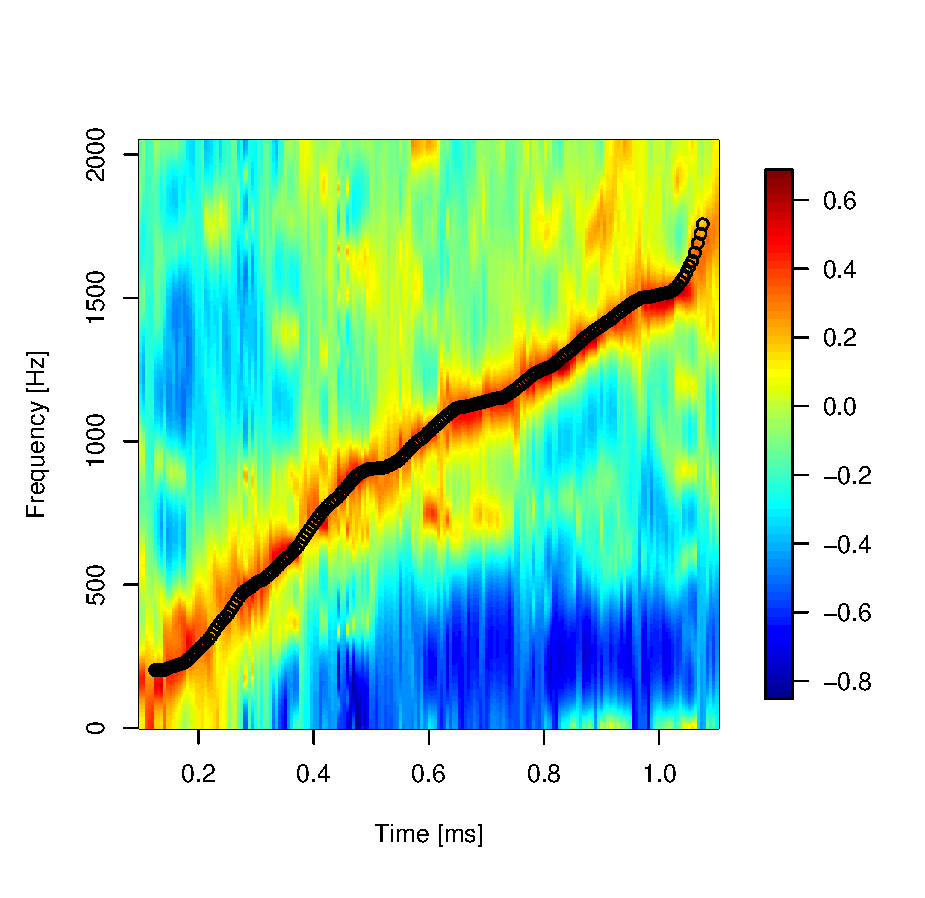
\includegraphics[width=0.5\textwidth]{plots/spectrogram}
 \caption{Spectrogram of the GW signal {\texttt s20S} sampled at \unit[4096]{Hz}.
   The spectrogram is obtained using a data streach of 200 samples overlapping at 90\%
   with each other. The open circles track the ridge $m(t) $ of the $\mbox{}^2 g_2$-mode. } \label{fig:spectrogram}
\end{figure}

We collect the instantaneous frequency $f(t_i)$ corresponding to the ridge $m(t_i)$ for
the midpoint $t_i$ of each local time interval of the spectrogram and interpolate $f(t)$
for values in between $t_i$. We then use our model given by Eq.~\eqref{eq:model1} to obtain
estimates of the time evolution of the ratio together with 95\% confidence intervals.
An example is given in Figure \ref{fig:ratio} where the red triangles are the point estimates and
the grey bands represent 95\% confidence bands. The size of the red triangles is proportional to the magnitude of the $\mbox{}^2 g_2$-mode frequency estimates.
Note that as the frequency of the $\mbox{}^2 g_2$-mode becomes higher our estimates show more uncertainty (bigger intervals) because our model allows for heterogeneous variance. Ratio values
computed using the mass and radius values obtained from the simulation code (i.e.~the true values)
are shown in black. In this example of a noise-free GW signal the coverage of our 95\% confidence band is 100\%
of the true values. In the next section we investigate the performance of the reconstruction of $r(t)$ when the GW
signal is embedded in noise. We also note that despite we have only explicitely shown results for the GW signal of the {\texttt s20S} model the same conclusions hold for any of the other waveforms of our test set.

\begin{figure}
 \centering
 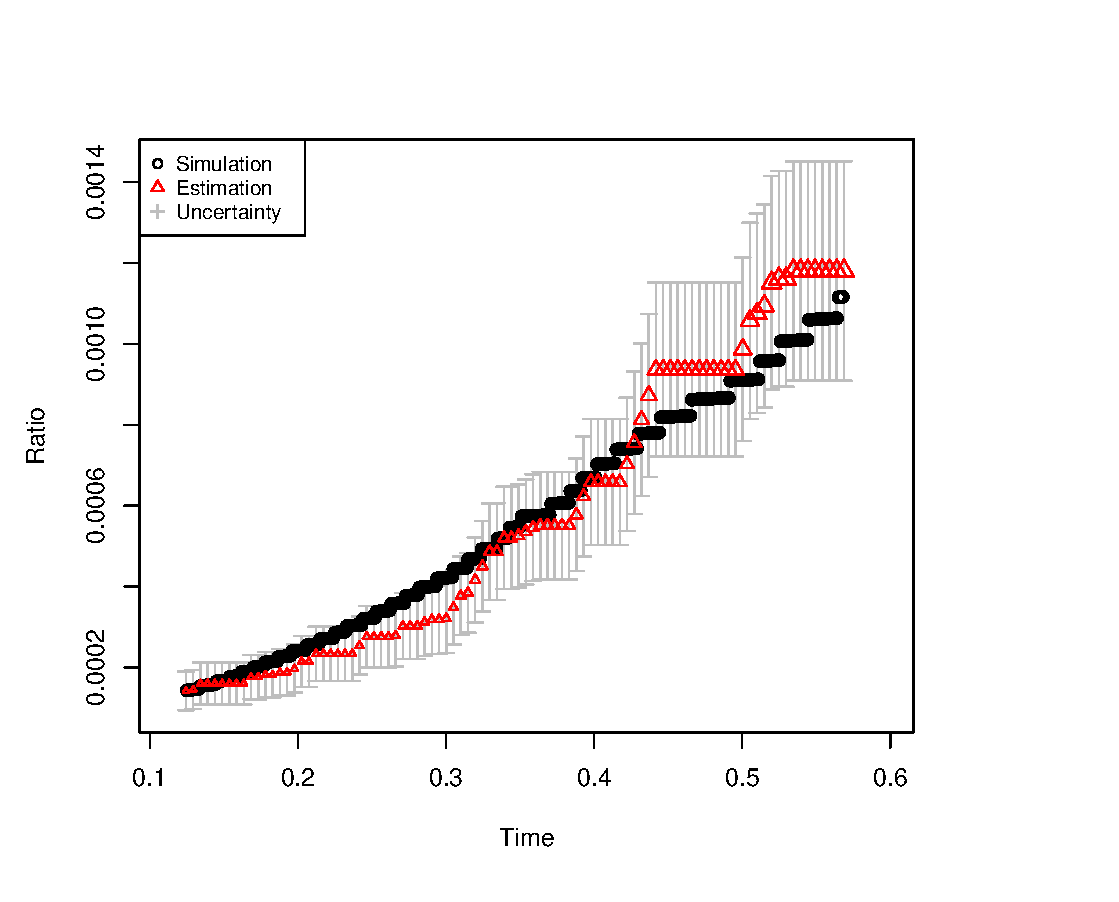
\includegraphics[width=0.5\textwidth]{plots/ratio}
 \caption{Comparison of the time evolution of the ratio $M_{\rm PNS}/R_{\rm PNS}^2$ estimated from the $\mbox{}^2 g_2$-mode of the {\texttt s20S} signal (shown by open triangles and by the 95\% confidence belt in grey) against the value derived from the PNS mass and radius given by the simulation code (shown by filled black circles). The size of the triangles are represented proportionally to the magnitude of the $\mbox{}^2 g_2$-mode frequency estimates.}
 \label{fig:ratio}
\end{figure}



\input{noisestudy}
\input{discussion}


\bigskip\noindent\textit{Acknowledgments} ---

%\bibliographystyle{unsrt}
\bibliography{biblio}


\end{document}
